\documentclass[a4paper,12pt]{report} % modello del documento
% \usepackage[top=1.8cm, bottom=2cm, left=2cm, right=2cm]{geometry} % margini aumentati
\usepackage[toc,page]{appendix}
\usepackage[italian]{babel} % imposta lingua
\usepackage[babel]{csquotes} % imposta lingua
\usepackage[utf8]{inputenc} % imposta lingua
\usepackage[T1]{fontenc} % imposta lingua
\usepackage{amsmath, amssymb, amsfonts} % pachetto per formule
% \usepackage[parfill]{parskip} % non si dovrebbe fare, ma sostituisce le rientranze dei paragrafi con interlinea
\usepackage{listings} % per poter far riconoscere e colorare codice 
\usepackage{subfig}
\usepackage{xcolor} % pacchetto per testo colorato
\usepackage{float} % pachetto per figure, per posizionamento
\usepackage{booktabs} % pacchetto per tabelle
\usepackage{graphicx, wrapfig} % pachetto per tabelle
\usepackage{tcolorbox} % riquadri colorati
\usepackage[Listato]{algorithm} % pseudocodice
\usepackage{algpseudocode} % pseudocodice
\usepackage[hidelinks]{hyperref} % indice e riferimenti cliccabili e senza riquadro rosso
\frenchspacing %spaziatura italiana per accenti
\usepackage[colorinlistoftodos,prependcaption,textsize=tiny]{todonotes} % note TODO
\usepackage{blindtext} %loreipsum
% CONFIGURAZIONE LINK E RIFERIMENTI
\hypersetup{%
	pdfpagemode={UseOutlines},
	bookmarksopen,
	pdfstartview={FitH},
	colorlinks,
	linkcolor={black}, %COLORE DEI RIFERIMENTI AL TESTO
	citecolor={blue}, %COLORE DEI RIFERIMENTI ALLE CITAZIONI
	urlcolor={blue} %COLORI DEGLI URL
}

\usepackage{color} %definizione colori
\definecolor{dkgreen}{rgb}{0,0.6,0}
\definecolor{gray}{rgb}{0.5,0.5,0.5}
\definecolor{mauve}{rgb}{0.58,0,0.82}
\lstset{%
	frame=tb,
	language=Python,
	aboveskip=3mm,
	belowskip=3mm,
	showstringspaces=false,
	columns=flexible,
	basicstyle=\ttm,
	numbers=none,
	numberstyle=\tiny\color{gray},
	keywords=[2]{self},
	keywordstyle=\color{deepblue},
	keywordstyle={[2]\color{deepblue}},
	commentstyle=\color{dkgreen},
	stringstyle=\color{mauve},
	breaklines=true,
	breakatwhitespace=true,
	tabsize=3,
	showstringspaces=false
}{}

\begin{document} %inizio del documento, va chuso alla fine

\title{Utilizzo di reti bayesiane in supporto alla diagnosi di patologie che portano alla sindrome del \textit{Blue Baby}} 
\author{Matteo Mistri 808097\\ Daniele Maria Papetti 808027}

\maketitle %comando di creazione della prima pagina
\tableofcontents %comando per creare l'indice

\chapter{Introduzione}
Con la sindrome del \textit{Blue Baby} ci riferiamo ad un insieme variegato di condizioni anomale e a volte patologiche che si manifestano con la colorazione cianotica della pelle di un neonato.
L'obiettivo principale dei medici è quello di trovare quale tra le patologie, che possono portare al colorito blu della pelle, sia presente nel bambino, al fine di intervenire repentinamente e in modo mirato sulle cause. Per fare ciò, i medici hanno a disposizioni una serie di esami clinici da compiere, che permettono di rilevare i sintomi tipici di alcune malattie che sono anche causa della sindrome in questione. Analizzando i risultati di questi test, gli specialisti sono in grado di restringere le possibili malattie che affliggono il neonato, individuando così la causa più probabile del colorito anomalo della pelle.

Nel nostro caso, alcuni ricercatori hanno lavorato a stretto contatto con medici ed esperti e sono riusciti a produrre una rappresentazione delle rete di dipendenza delle malattie che causano il fenomeno (Spiegelhalter \textit{et al.}, Statistical science 1993). La rete prodotta, riportata in Figura \ref{fig:paperstructure}, contiene una serie di sintomi, esami e dati sul paziente (\textit{i.e.}, sintomatologia e relativa presentazione) che permettono di modificare la probabilità che una malattia sia presente nell'infante. Tale modello assume che non coesista più di una patologia in ogni paziente che causi la sindrome studiata. Possiamo vedere come i nodi della rete si dispongano secondo una struttura ad albero; in particolare, i figli del nodo \textit{Disease} sono situazioni patologiche manifestate in alcune delle malattie che possono causare la sindrome in analisi. I figli di questi nodi sono o nuove situazioni patologiche causalmente collegate alle precedenti, o esami che permettono di accertarne la presenza (\textit{e.g.}, il mescolamento del sangue a livello cardiaco, rappresentata dal nodo \textit{CardiacMixing}, causa un'ipossia polmonare, rappresentata dal nodo \textit{HypoxiaInO2}, che è un figlio del nodo precedente).
 
 \begin{figure}
 	\centering
 	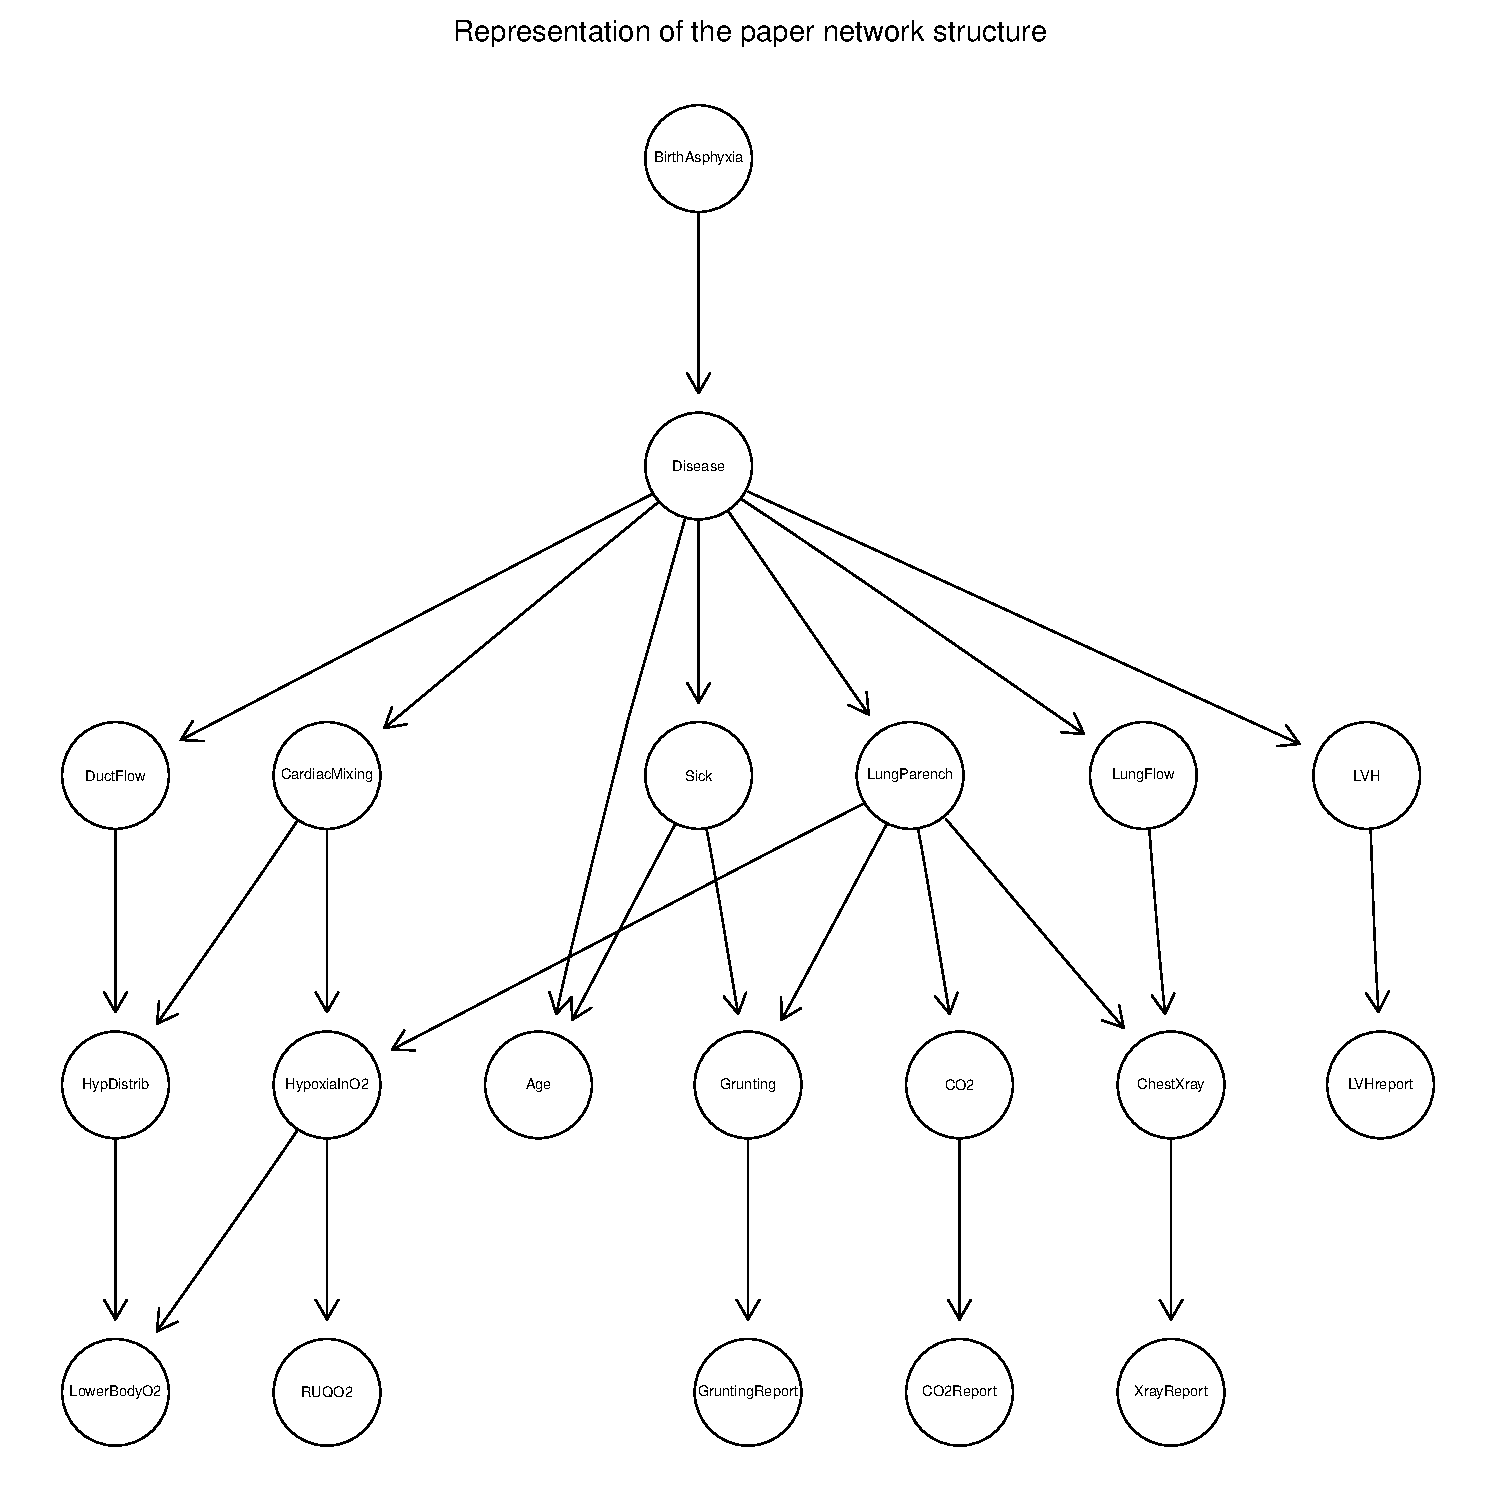
\includegraphics[width=1\linewidth]{images/paper_structure}
 	\caption{Rappresentazione della rete prodotta dai ricercatori, in collaborazione con medici ed esperti. Ogni nodo rappresenta un sintomo, un esame o un dato del paziente.}
 	\label{fig:paperstructure}
 \end{figure}

\section{Obiettivi}
Nel nostro lavoro, abbiamo voluto studiare se fosse possibile inferire la struttura della rete a partire da un dataset contenete evidenze dei nodi della rete in casi accertati (e non) della sindrome del \textit{BlueBaby}. Cercheremo poi di capire se vi siano dei nodi che sono condizionalmente indipendenti da altri nodi data l'evidenza di un insieme di variabili, in modo da consentire la riduzione del numero di esami necessari al fine di ottenere una diagnosi accurata. Vaglieremo infine la possibilità di utilizzare la rete invertendo le relazioni da causalità, analizzando i risultati ottenuti e comparandoli quelli della rete proposta. Ci siamo inoltre posti l'obiettivo di produrre un'interfaccia grafica nella quale il medico può inserire il valore dei nodi di cui ha conoscenza e ottenere una stima della probabilità della presenza delle varie malattie nel neonato.
\chapter{Inferenza della struttura}
\section{Analisi delle tecniche utilizzate}
\label{sec:misure}
Il nostro obiettivo principale è quello di verificare se sia possibile apprendere la struttura della rete a partire da un dataset contenente i dati di $10000$ pazienti con la sindrome del \textit{BlueBaby}. Al fine di fare ciò, sono state considerate due differenti approcci, ovvero la tecnica \texttt{Hill Climb} e la tecnica \texttt{Tabù Search}. Entrambe le tecniche di analizzate sono basate su un processo meta-euristico di ottimizzazione di una funzione di score. Documentandoci sulle due tecniche prese in esame, ed effettuando alcuni test preliminari, abbiamo notato come le performance della ricerca Tabù siano superiori a quelle della prima tecnica citata, in quanto la seconda permette di evitare lo stallo della ricerca nei minimi locali.\\
\begin{table}[t!]
	\centering
	\caption{Differenti funzioni di score a confronto. La colonna \textit{Archi paper} mostra il numero di archi presenti nella rete proposta dal paper ma non presente nel modello generato. Viceversa, l'ultima colonna indica il numero di archi presenti nel modello appreso ma non presenti nella rete del paper.}
	\begin{tabular}{|c|c|c|c|c|}
		\hline 
		Funzione & Archi generati  & Archi comuni & Archi paper & Archi appreso \\ 
		\hline 
		aic & 32 & 24 & 1 & 8 \\ 
		\hline 
		bic & 26 & 18 & 7 & 8 \\ 
		\hline 
		bde & 26 & 21 & 4 & 5 \\ 
		\hline 
		bds & 26 & 18 & 7 & 8 \\ 
		\hline 
		mbde & 26 & 21 & 4 & 5 \\ 
		\hline 
		bdla & 26 & 21 & 4 & 5 \\ 
		\hline 
		k2 & 25 & 24 & 1 & 1 \\ 
		\hline 
	\end{tabular} 
	\label{tab:score}
\end{table}
Abbiamo quindi approfondito le possibili funzioni di score disponibili per la ricerca Tabù, confrontando la rete prodotta con quella fornita dal \textit{paper} di riferimento. I risultati ottenuti, proposti in Tabella \ref{tab:score}, mostrano come molte misure ottengano performance simili, mentre quella che si distingue dalle altre risulta essere la funzione \texttt{k2}, che stima correttamente il numero di archi, inserendo un solo arco in posizione non ottimale.

La Figura mostra la rappresentazione prodotta dall'algoritmo \texttt{Tabù Search} con la funzione di score \texttt{k2}; confrontando questa struttura con quella proposta in Figura \ref{fig:paperstructure}, notiamo come l'unico arco differente sia quello che collega i nodi \textit{Age} e \textit{Sick}.

\begin{figure}
	\centering
	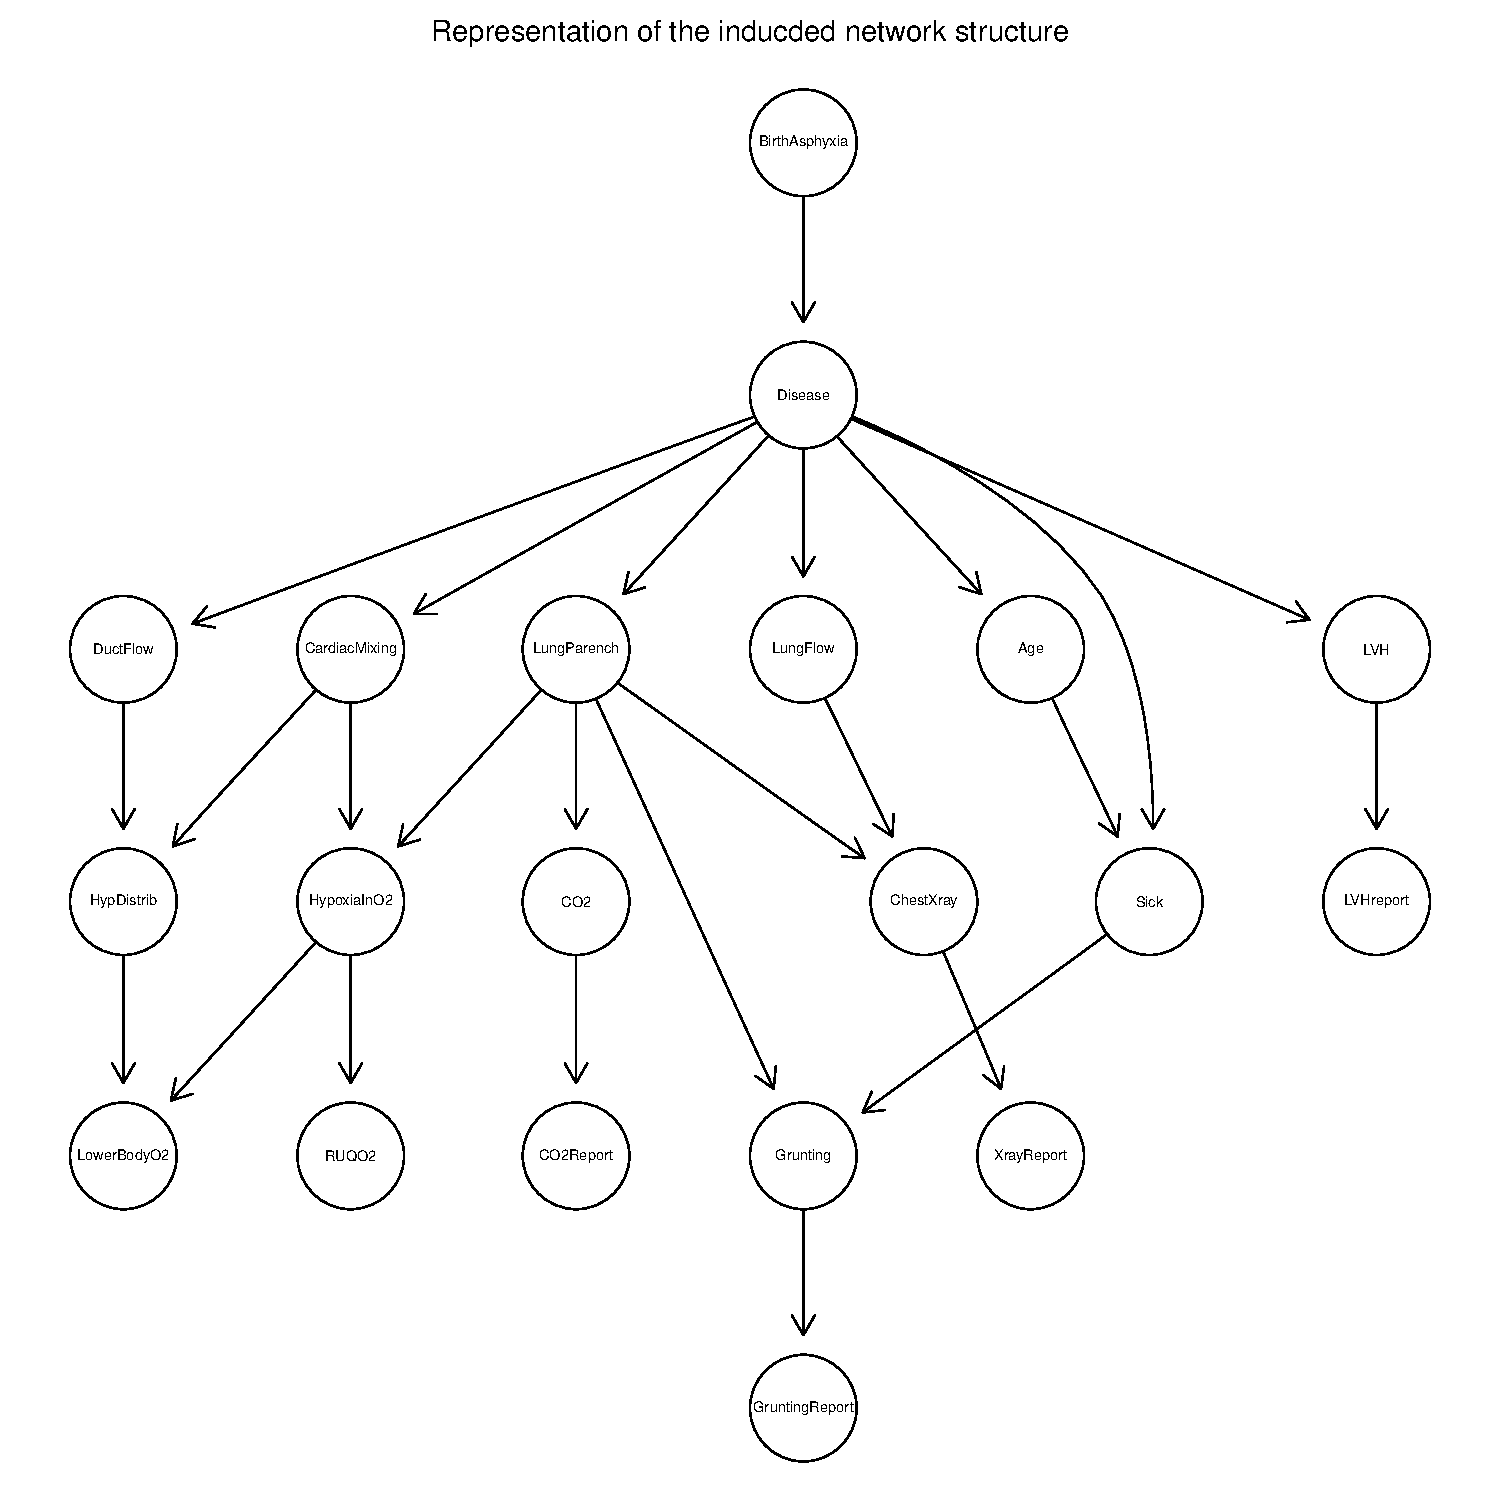
\includegraphics[width=.9\linewidth]{images/induced_structure}
	\caption{Rappresentazione della struttura appresa con la ricerca di Tabù e la funzione di score \texttt{k2}}
	\label{fig:inducedstructure}
\end{figure}

\newpage
\section{Misure di performance delle reti}
Una volta indotta la struttura della rete con il metodo illustrato nella Sezione \ref{sec:misure}, abbiamo deciso di valutare le capacità predittive della reti proposte per quanto riguarda la predizione della variabile \textit{Disease}. Per fare ciò, abbiamo deciso di effettuare un'operazione di \textit{10-times 10-fold coross validation}, al fine di garantire la significatività statistica dei risultati ottenuti. In ogni fold, per le due reti vengono stimate le CPT di ogni nodo utilizzando il $90\%$ del dataset; viene poi utilizzata la tecnica \textit{likelihood weighting}, generando 500 sample per ogni nuova osservazione, per determinare il valore del nodo \textit{Disease} associato ad una particolare istanza.

Le performance ottenute, riportate nelle Figure \ref{fig:paperperformance} e \ref{fig:inducedperformance}, calcolate come la media delle dieci ripetizioni del processo di \textit{cross validation}, risultano essere molto simili. Al fine di indagare se le performance dei due modelli proposti fossero statisticamente differenti, sono stati eseguiti dei test di significatività \textit{t-student}; i risultati ottenuti hanno mostrato come le performance medie dei due modelli siano di fatto equivalenti, a meno di un errore attribuibile al caso.
\begin{figure}
	\centering
	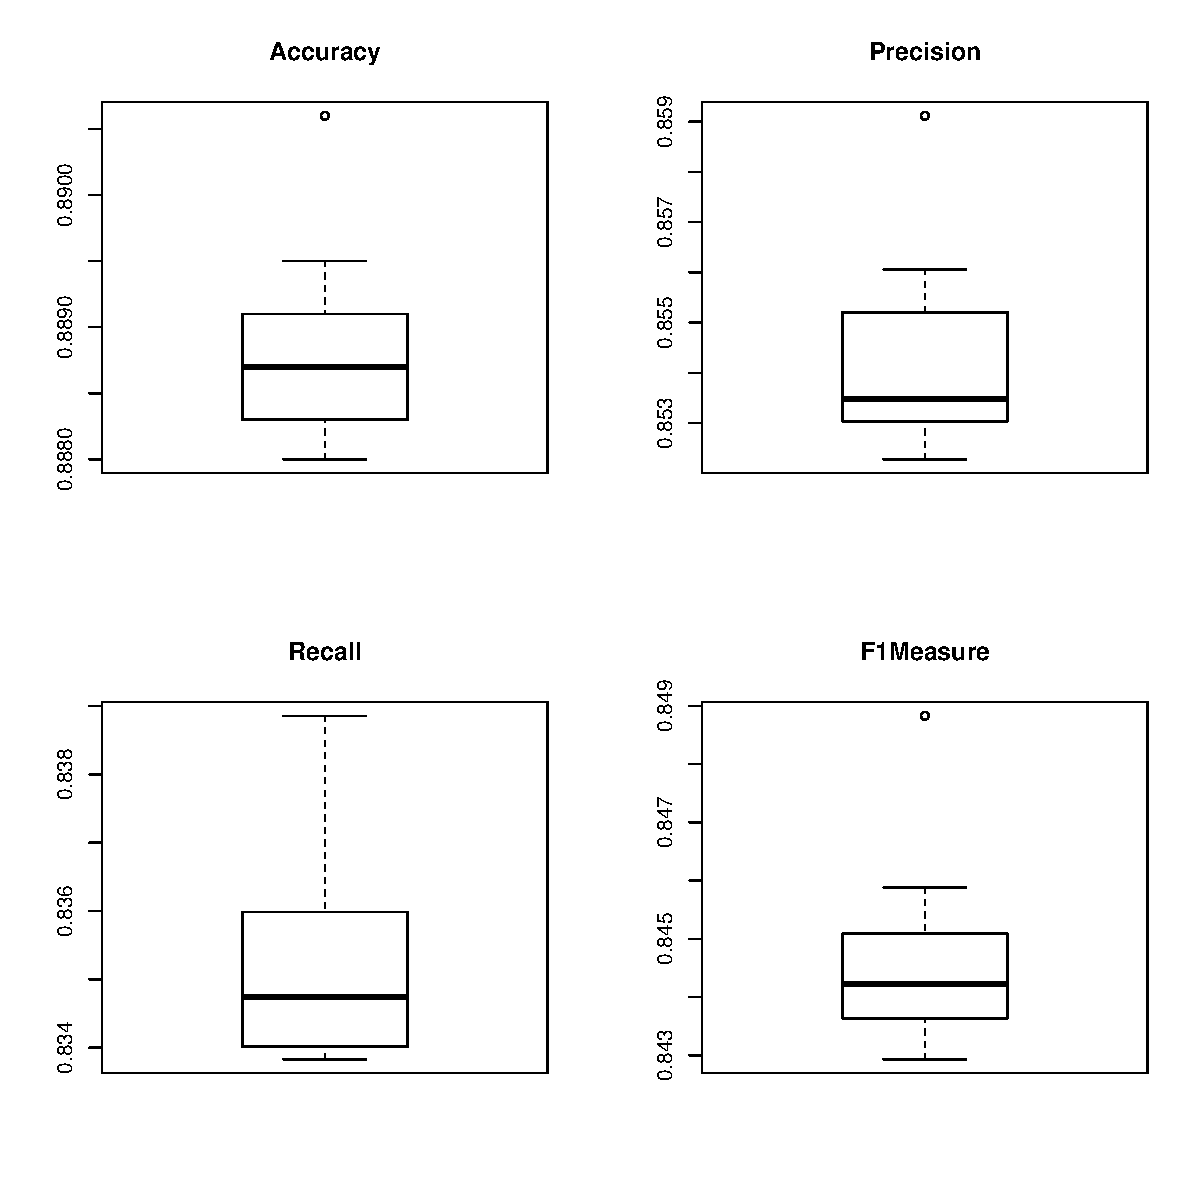
\includegraphics[width=0.7\linewidth]{images/paper_performance}
	\caption{Performance ottenute dalla rete proposta dal paper.}
	\label{fig:paperperformance}
\end{figure}
\begin{figure}
	\centering
	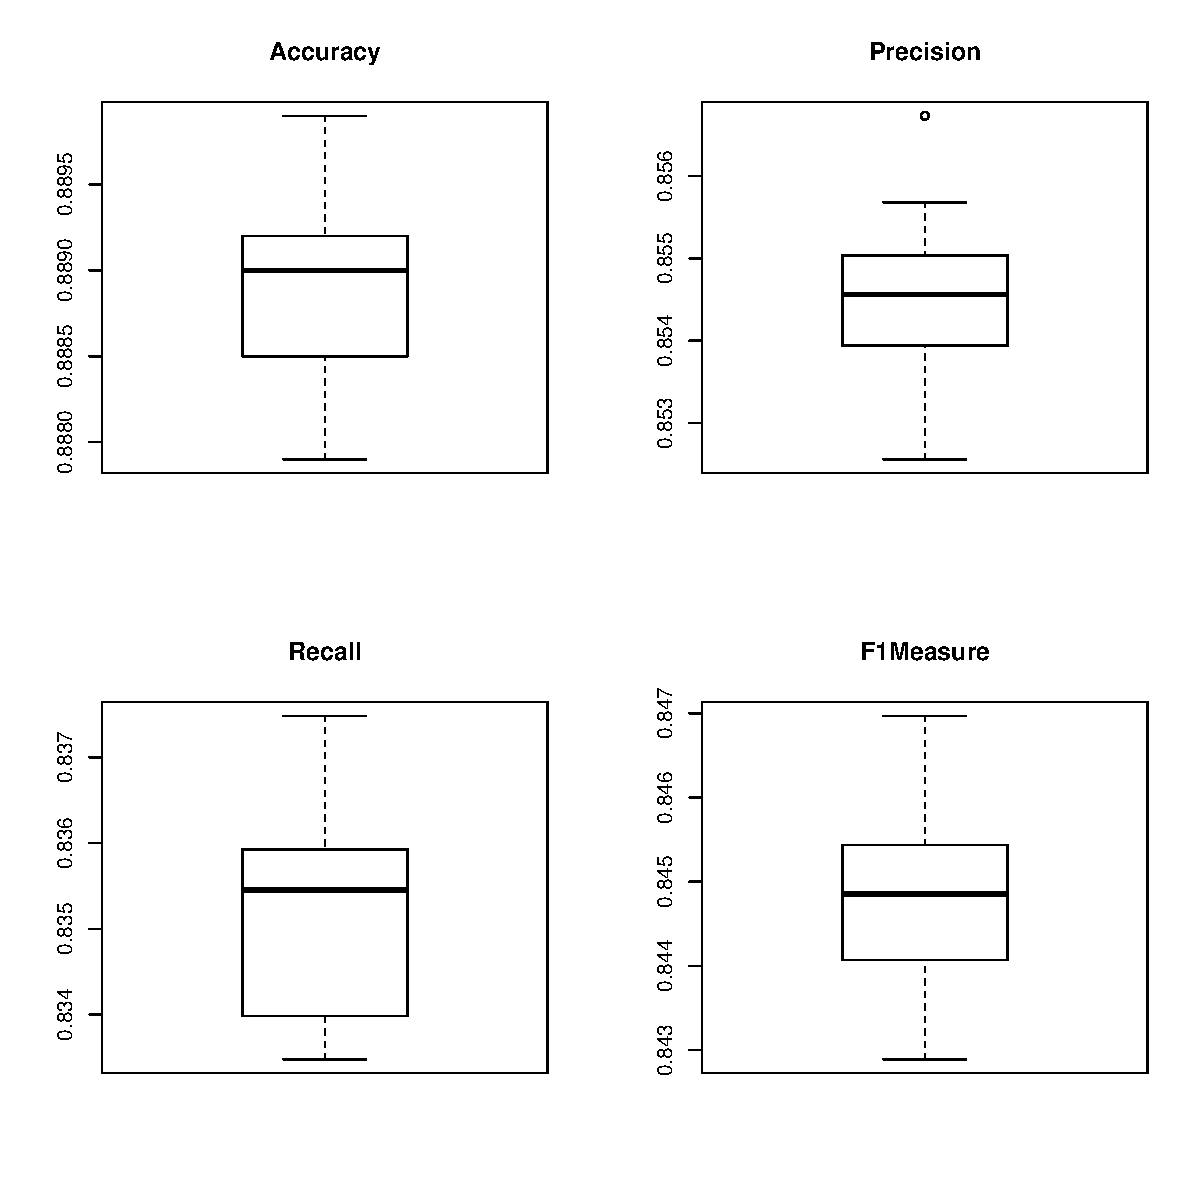
\includegraphics[width=0.7\linewidth]{images/induced_performance}
	\caption{Performance ottenute dalla rete appresa dal dataset.}
	\label{fig:inducedperformance}
\end{figure}
Questo è una conferma di come la struttura appresa dal dataset utilizzato sia valida e in grado di predire valori per il nodo \textit{Disease} in modo efficace; la presenza di un'unico arco in posizione differente non ha quindi impattato negativamente sulle performance predittive.

Analizzando più specificamente il dominio di applicazione, abbiamo deciso di ripetere le operazioni di inferenza del valore di \textit{Disease} fornendo non più un'evidenza completa delle variabili della rete, bensì fornendo solo di quei nodi che abbiamo ritenuto essere effettivamente osservabili dai medici, ovvero i dati del paziente e i risultati degli esami.\\
Le performance ottenute dalle due reti, riportate nelle Figure \ref{fig:paperperformancehalf} e \ref{fig:inducedperformancehalf}, sono, come ci aspettavamo, sensibilmente inferiori; ciononostante, le performance dei due modelli risultano nuovamente statisticamente non dissimili, avallando ulteriormente la tesi che la struttura appresa dai dati sia valida.\\
\begin{figure}
	\centering
	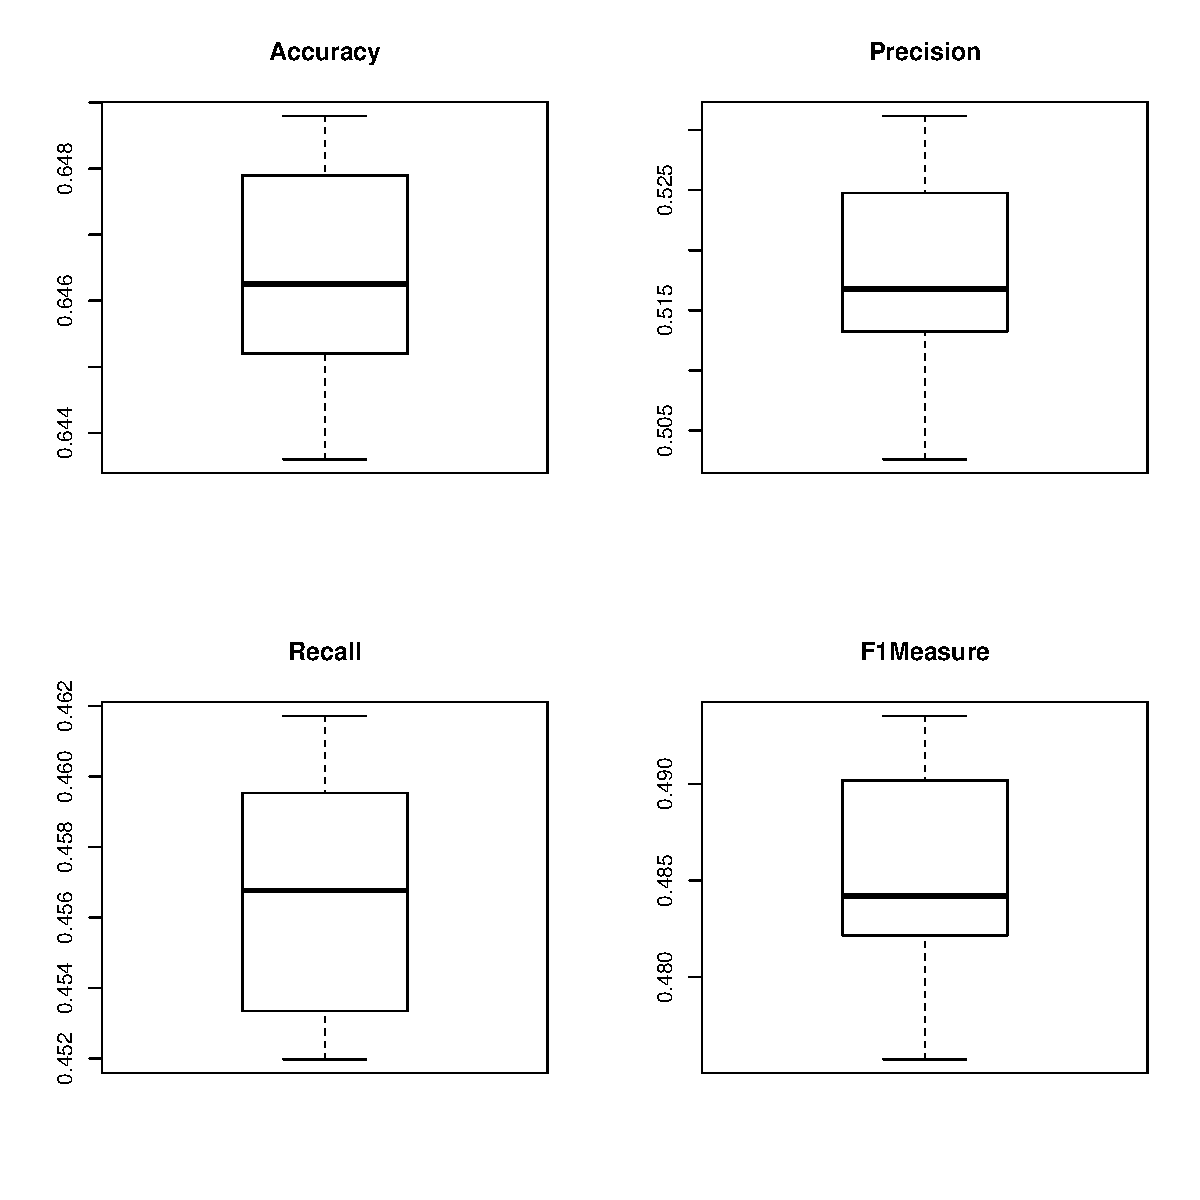
\includegraphics[width=0.7\linewidth]{images/paper_performance_half}
	\caption{Performance ottenute dalla rete proposta dal paper.}
	\label{fig:paperperformancehalf}
\end{figure}
\begin{figure}
	\centering
	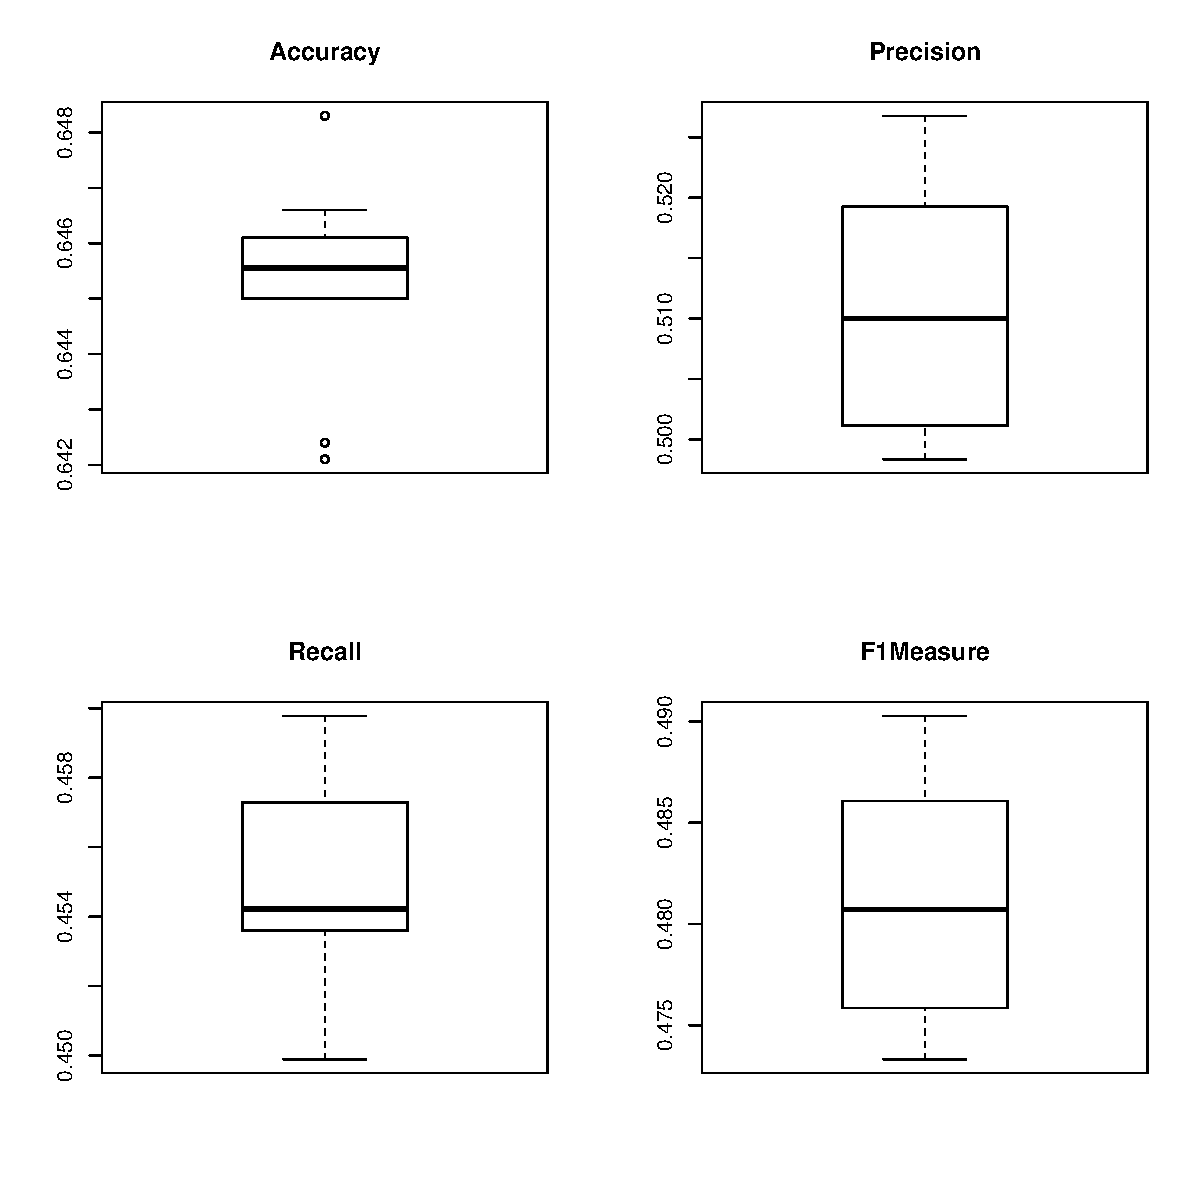
\includegraphics[width=0.7\linewidth]{images/induced_performance_half}
	\caption{Performance ottenute dalla rete appresa dal dataset.}
	\label{fig:inducedperformancehalf}
\end{figure}



\chapter{Conclusioni e sviluppi futuri}



\end{document}
